% !TEX root = Projektdokumentation.tex
\appendix
\section{Anhang}
\label{sec:Anhang}

\subsection*{Abkürzungsverzeichnis}
\label{sec:Abkürzungsverzeichnis}
\addcontentsline{toc}{subsection}{Abkürzungsverzeichnis}
\begin{acronym}[WWWWW]
	% \acro{TAL}{Tech Accelerator Leipzig}
	\acro{SSH}{Secure Shell}
	\acro{B and TCL}{Business \& Technology Center Leipzig}
	\acro{API}{Application Programming Interface}
	\acro{LDAP}{Lightweight Directory Access Protocol}
	\acro{OIDC}{OpenID Connect}
	\acro{CPU}{Control Processing Unit}
  \acro{RAM}{Random Access Memory}
  \acro{CLI}{Command Line Interface}
  \acro{A}{Adresse}
  \acro{CNAME}{Canonical name}
  \acro{DNS}{Domain Name System}
  \acro{HSTS}{HTTP Strict Transport Security}
	\acro{ISMS}{Informationssicherheits-Managementsystem}
	\acro{BSI}{Bundesamt für Sicherheit in der Informationstechnik}
	\acro{TOTP}{Time-based One-time Password}
	\acro{SSO}{Single-Sign On}
	\acro{MFA}{Multi Faktor Authentifizierung}
	\acro{IDE}{Integrated Development Environment}
	\acro{TCO}{Total Cost of Ownership}
\end{acronym}
\cleardoublepage

\subsection*{Begriffserklärung}
\label{sec:Begriffserklärung}
\addcontentsline{toc}{subsection}{Begriffserklärung}
\begin{description}
  \item[SSH] Secure Shell - Netzwerkprotokoll zur sicheren Datenübertragung
  \item[B and TCL] Business \& Technology Center Leipzig - Deloitte Standort in Leipzig
  \item[API] Application Programming Interface - Schnittstelle zur Kommunikation zwischen Softwareanwendungen
  \item[LDAP] Lightweight Directory Access Protocol - Protokoll zum Abrufen von Informationen aus einem Verzeichnisdienst
  \item[OIDC] OpenID Connect - Authentifizierungsprotokoll für Webanwendungen
  \item[CPU] Control Processing Unit - zentrale Recheneinheit eines Computers
  \item[RAM] Random Access Memory - Speichertyp, der Daten temporär speichert und schnell darauf zugreifen kann
  \item[CLI] Command Line Interface - textbasierte Benutzeroberfläche zur Interaktion mit einem Computersystem
  \item[A] Address (DNS Resource Record) - DNS-Ressourceneintrag, der eine IPv4-Adresse mit einem Domainnamen verknüpft
  \item[CNAME] Canonical name - Eintrag in DNS, der eine Alias-Beziehung zwischen zwei Domainnamen darstellt
  \item[DNS] Domain Name System - System zur Übersetzung von Domainnamen in IP-Adressen
  \item[HSTS] HTTP Strict Transport Security - Sicherheitsmechanismus, der Webanwendungen vor bestimmten Angriffen schützt
  \item[ISMS] Informationssicherheits-Managementsystem - Rahmenwerk zur Informationssicherheit in Organisationen
  \item[BSI] Bundesamt für Sicherheit in der Informationstechnik - deutsche Behörde für IT-Sicherheit
  \item[TOTP] Time-based One-time Password - Einmalpasswort, das basierend auf der Zeit generiert wird
  \item[SSO] Single-Sign On - Authentifizierungsverfahren, bei dem sich Benutzer einmal anmelden, um auf verschiedene Dienste zuzugreifen
  \item[MFA] Multi Faktor Authentifizierung - Authentifizierungsverfahren, das mehrere Methoden zur Bestätigung der Identität eines Benutzers verwendet
  \item[IDE] Integrated Development Environment - intelligente Entwicklungsumgebung für die Softwareentwicklung
  \item[TCO] Total Cost of Ownership - Gesamtkosten von Produktanschaffung und Nutzung
\end{description}
\cleardoublepage

\subsection{Gantt-Diagramm und Meilensteine}
\label{app:Gantt}
\includegraphicsKeepAspectRatio{Anhang/Gantt.pdf}{1}
\clearpage

\subsection{Detaillierte Zeitplanung}
\tabelleAnhang{ZeitplanungKomplett}
\clearpage

\subsection{Use Case-Diagramm}
\label{app:UseCase}
\begin{figure}[htb]
  \centering
  \includegraphicsKeepAspectRatio{Anhang/UseCaseCloudInfra.png}{1}
  \caption{Use Case-Diagramm}
\end{figure}
\clearpage

\subsection{Sequenzdiagramm CLI Zugriff auf die Instanzen}
\label{app:Sequenzdiagramm CLI Zugriff auf die Instanzen}
\begin{figure}[htb]
  \centering
  \includegraphicsKeepAspectRatio{Anhang/SequenzDiagrammCLI.png}{1}
  \caption{Sequenzdiagramm}
\end{figure}
\clearpage

\subsection{Cloud-Infrastruktur}
\label{app:Cloud-Infrastruktur}
\begin{figure}[htb]
    \centering
    \includegraphicsKeepAspectRatio{Anhang/CloudInfra.png}{0.8}
    \caption{Cloud-Infrastruktur}
\end{figure}
\pagebreak

\subsection{docker-compose.yml}
\label{app:docker-compose.yml}
\includegraphicsKeepAspectRatio{Anhang/docker-compose.pdf}{0.9}

\subsection{.env}
\label{app:dotenv}
\includegraphicsKeepAspectRatio{Anhang/(.)env.pdf}{0.9}
\clearpage

\subsection{Docker-Befehle}
\label{app:dockercommands}
\begin{figure}[ht]
    \centering
    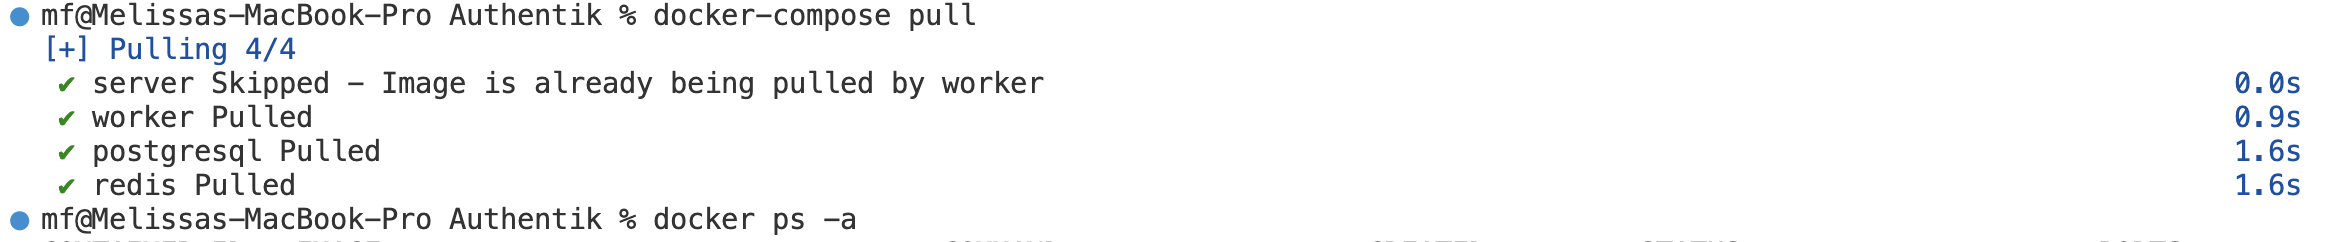
\includegraphics[scale=0.4]{Bilder/Authentik-Doc/DP_00_DockerPull.png}
    \caption{Docker Pull}
  \end{figure}
  
  \vspace{0.5cm} % Adjust vertical space as needed
  
  \begin{figure}[ht]
    \centering
    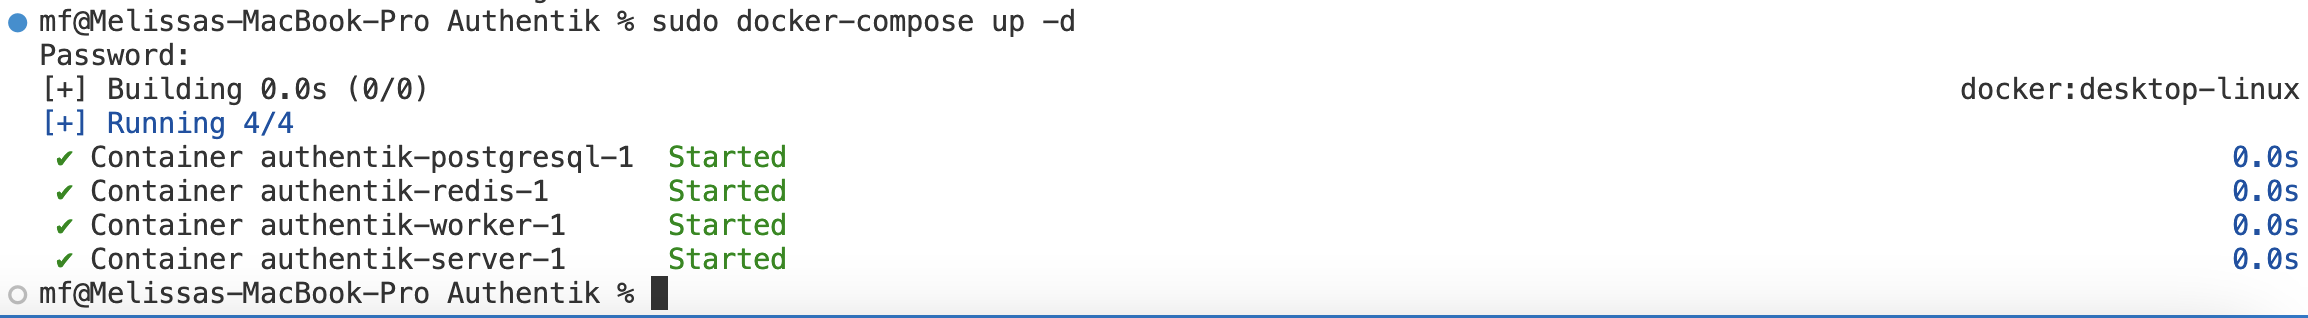
\includegraphics[scale=0.4]{Bilder/Authentik-Doc/DP_01_DockerComposeUp.png}
    \caption{Docker Compose Up}
  \end{figure}

\subsection{Proxy Host Konfiguration}
\label{app:ProxyHostConfig}
\includegraphicsKeepAspectRatio{Anhang/ProxyHostKonfiguration.pdf}{0.9}

\subsection{Authentik-Konfiguration}
\label{app:AuthentikConfig}
% 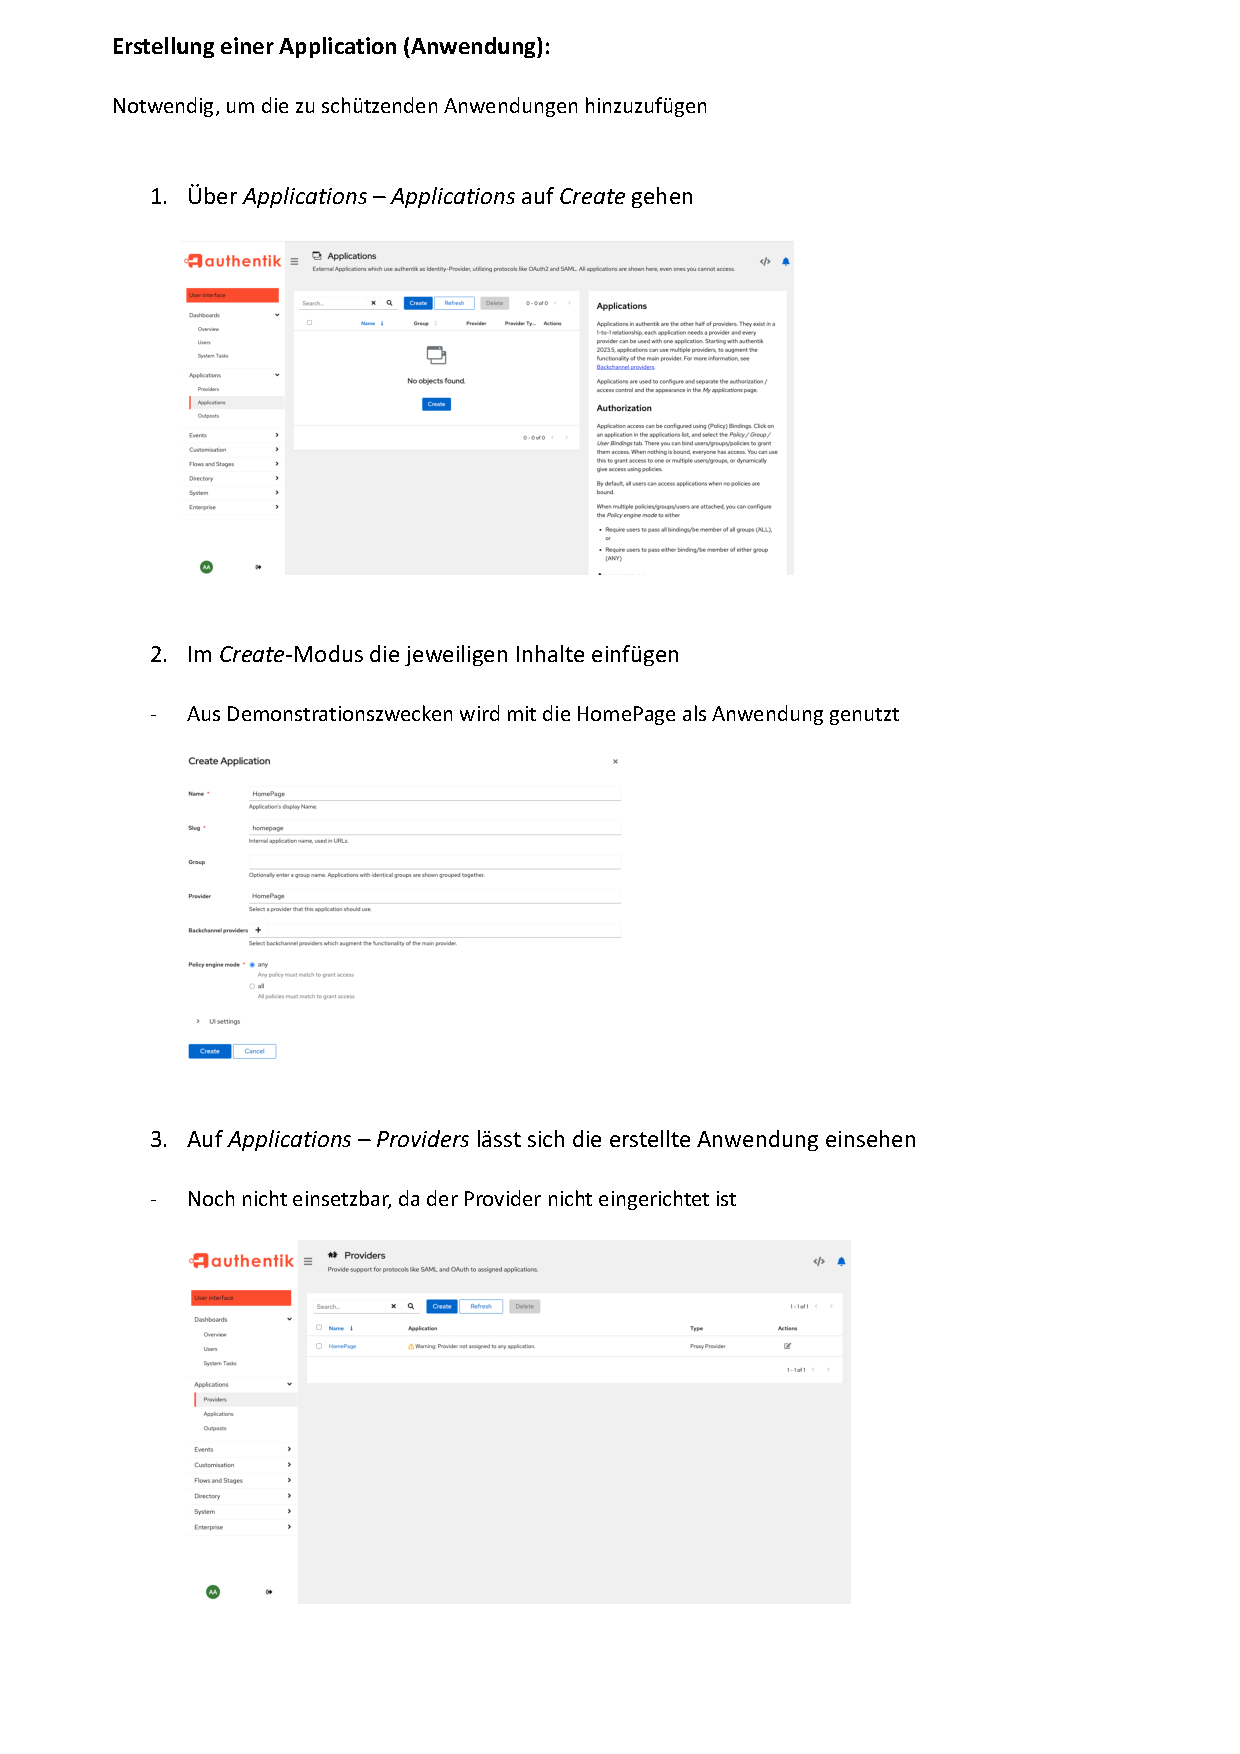
\includepdf[pages={1-3}, scale=0.9]{Anhang/Authentik-Konfiguration.pdf}
\includegraphicsKeepAspectRatio{Anhang/AuthentikKonfig1.png}{0.9}
\clearpage
\includegraphicsKeepAspectRatio{Anhang/AuthentikKonfig2.png}{0.9}
\clearpage
\includegraphicsKeepAspectRatio{Anhang/AuthentikKonfig3.png}{0.9}
\clearpage

\subsection{NGinx Konfiguration}
\label{app:CustomNGinxConfig}
\includegraphicsKeepAspectRatio{Anhang/Custom_NGinx_Configuration.pdf}{0.9}
\clearpage
\begin{figure}[htb]
    \centering
    \includegraphicsKeepAspectRatio{Bilder/Authentik-Doc/NS_03_ChangeIPInCustomNGinxConfig.png}{0.4}
    \captionbelow{Proxy Host Konfiguration - Einfügen des Code-Snippets in den Bereich \textbf{Advanced} 
    und erfolgt das Ändern der IP-Adresse mit dem zugehörigen Port}
\end{figure}

\subsection{TOTP-Einrichtung}
\label{sec:TOTPConfig}
\includegraphicsKeepAspectRatio{Anhang/TOTP-Einrichtung.pdf}{0.9}

\subsection{Benutzerdokumentation}
\label{app:Benutzerdokumentation}
\includegraphicsKeepAspectRatio{Anhang/Benutzerdokumentation.pdf}{0.9}

\subsection{Testprotokoll}
\label{app:Testprotokoll}
\includegraphicsKeepAspectRatio{Anhang/Test-Protokoll.pdf}{0.9}

\subsection{Übernahmeprotokoll}
\label{app:Übernahmeprotokoll}
\includegraphicsKeepAspectRatio{Anhang/Übernahme-Protokoll.pdf}{0.9}
\cleardoublepage

% Abbildungsverzeichnis ------------------------------------------------------
% \phantomsection
\listoffigures
\cleardoublepage

% Tabellenverzeichnis
\phantomsection
\listoftables
\cleardoublepage
% Literatur ------------------------------------------------------------------
\clearpage
\renewcommand{\refname}{Literaturverzeichnis}
\bibliography{Bibliographie}
\bibliographystyle{Allgemein/natdin} % DIN-Stil des Literaturverzeichnisses
% !TEX root = Projektdokumentation.tex
\clearpage
\addsec{Eidesstattliche Erklärung}

% Hinweis: die eidesstattliche Erklärung ist ggfs. an die Richtlinie der IHK anzupassen

Ich, \autorName, versichere hiermit, dass ich meine \textbf{\betreff} mit dem
Thema
\begin{quote}
\textit{\kompletterTitel}
\end{quote}
selbständig verfasst und keine anderen als die angegebenen Quellen und Hilfsmittel benutzt habe,
wobei ich alle wörtlichen und sinngemäßen Zitate als solche gekennzeichnet habe. Die Arbeit
wurde bisher keiner anderen Prüfungsbehörde vorgelegt und auch nicht veröffentlicht.\\[6ex]

\abgabeOrt, den \abgabeTermin


\rule[-0.2cm]{5.5cm}{0.5pt}

\textsc{\autorName}

\cleardoublepage